\begin{mainquestion}{controlledsourcegain}{Your Choice}
Consider the circuit below:

\begin{center}
    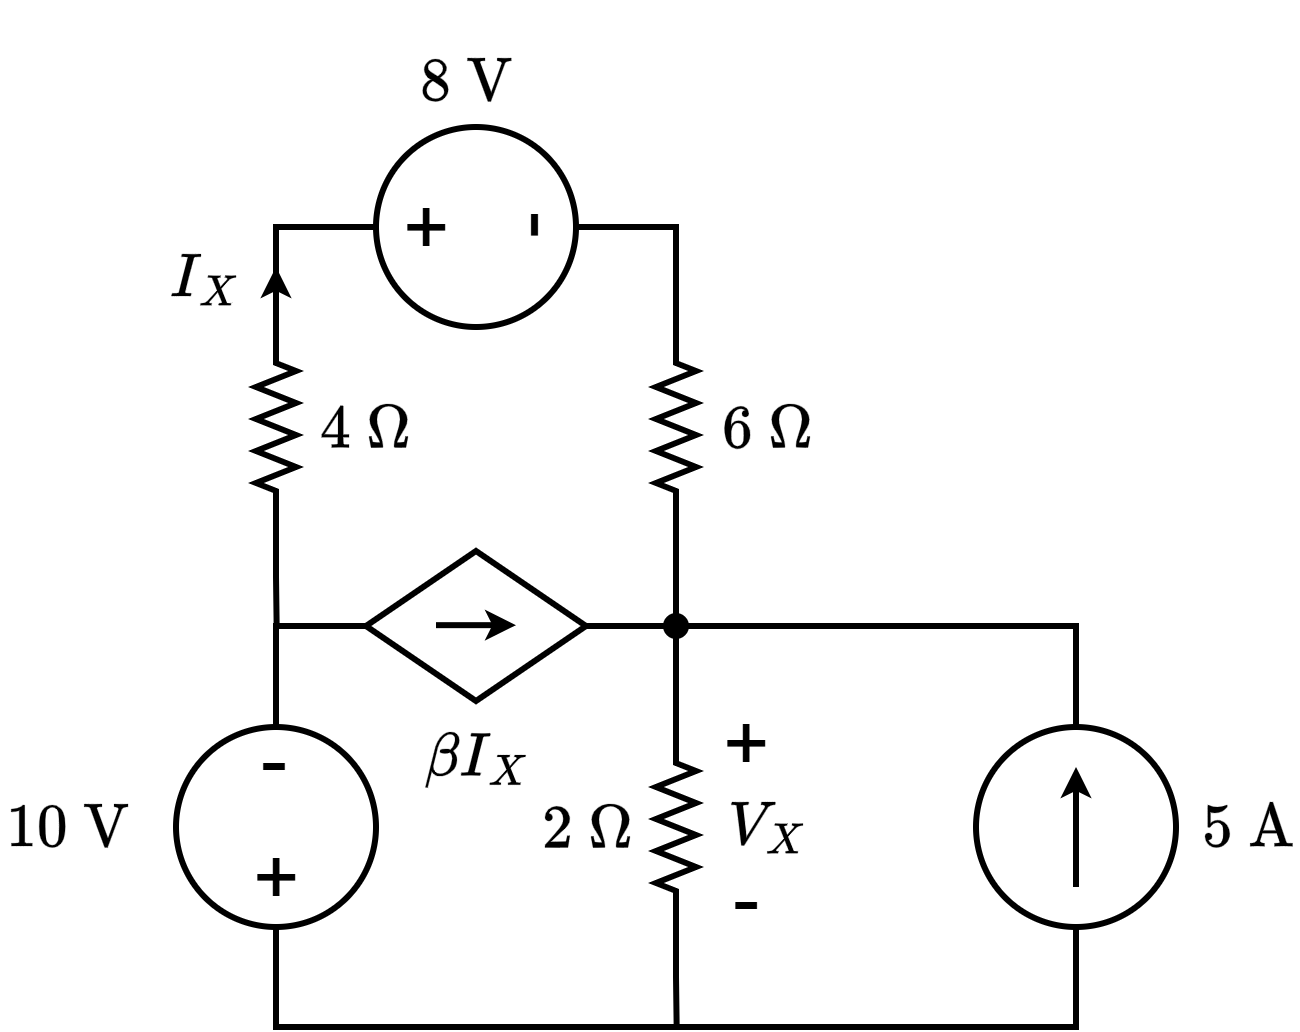
\includegraphics[width=0.8\textwidth]{super_cir.png}
\end{center}

\begin{partquestion}{formulavx}{Use a method of your choice to solve for $V_X$ in terms of the current gain $\beta$}
\begin{answer}

Let's evaluate our options. We could use:
\begin{enumerate}
    \item \textbf{Mesh Analysis:} There are 3 meshes, so in the worst worse case we may have 3 KVL equations to solve (If you are familiar with the concept of a supermesh, we could reduce this to one KVL equation)
    \item \textbf{Nodal Analysis:} There are 5 nodes, so in the worst case we may have 4 KCL equations to solve. (If you are familiar with the concept of a supernode, we could reduce this to one KCL equation)
    \item \textbf{Superposition:} There are 3 sources, and we'll have to solve for $V_X$ in the presence of the dependent current source. Worst case three smaller problems.
    \item \textbf{Source Transformations:} Definitely possible, but we'd need to think carefully on how to account for the dependent current source.
\end{enumerate}

Let's use superposition for now given it's a straight forward technique based on our current knowledge. Superposition tells us that we can consider the effect of each independent source individually. We can do this by disabling all but one of the independent sources (open current sources, short voltage sources) and solving for $V_X$. Keep in mind you shouldn't deactivate any dependent sources. Then we can add up all the results and we should get the final value of $V_X$.
\bigskip

\textbf{5 A source only:} short the 10 V and 8V sources. The \qty{4}{\ohm} and \qty{6}{\ohm} resistors can be combined and the whole circuit can be redrawn to look like a current divider as seen below:
\begin{center}
    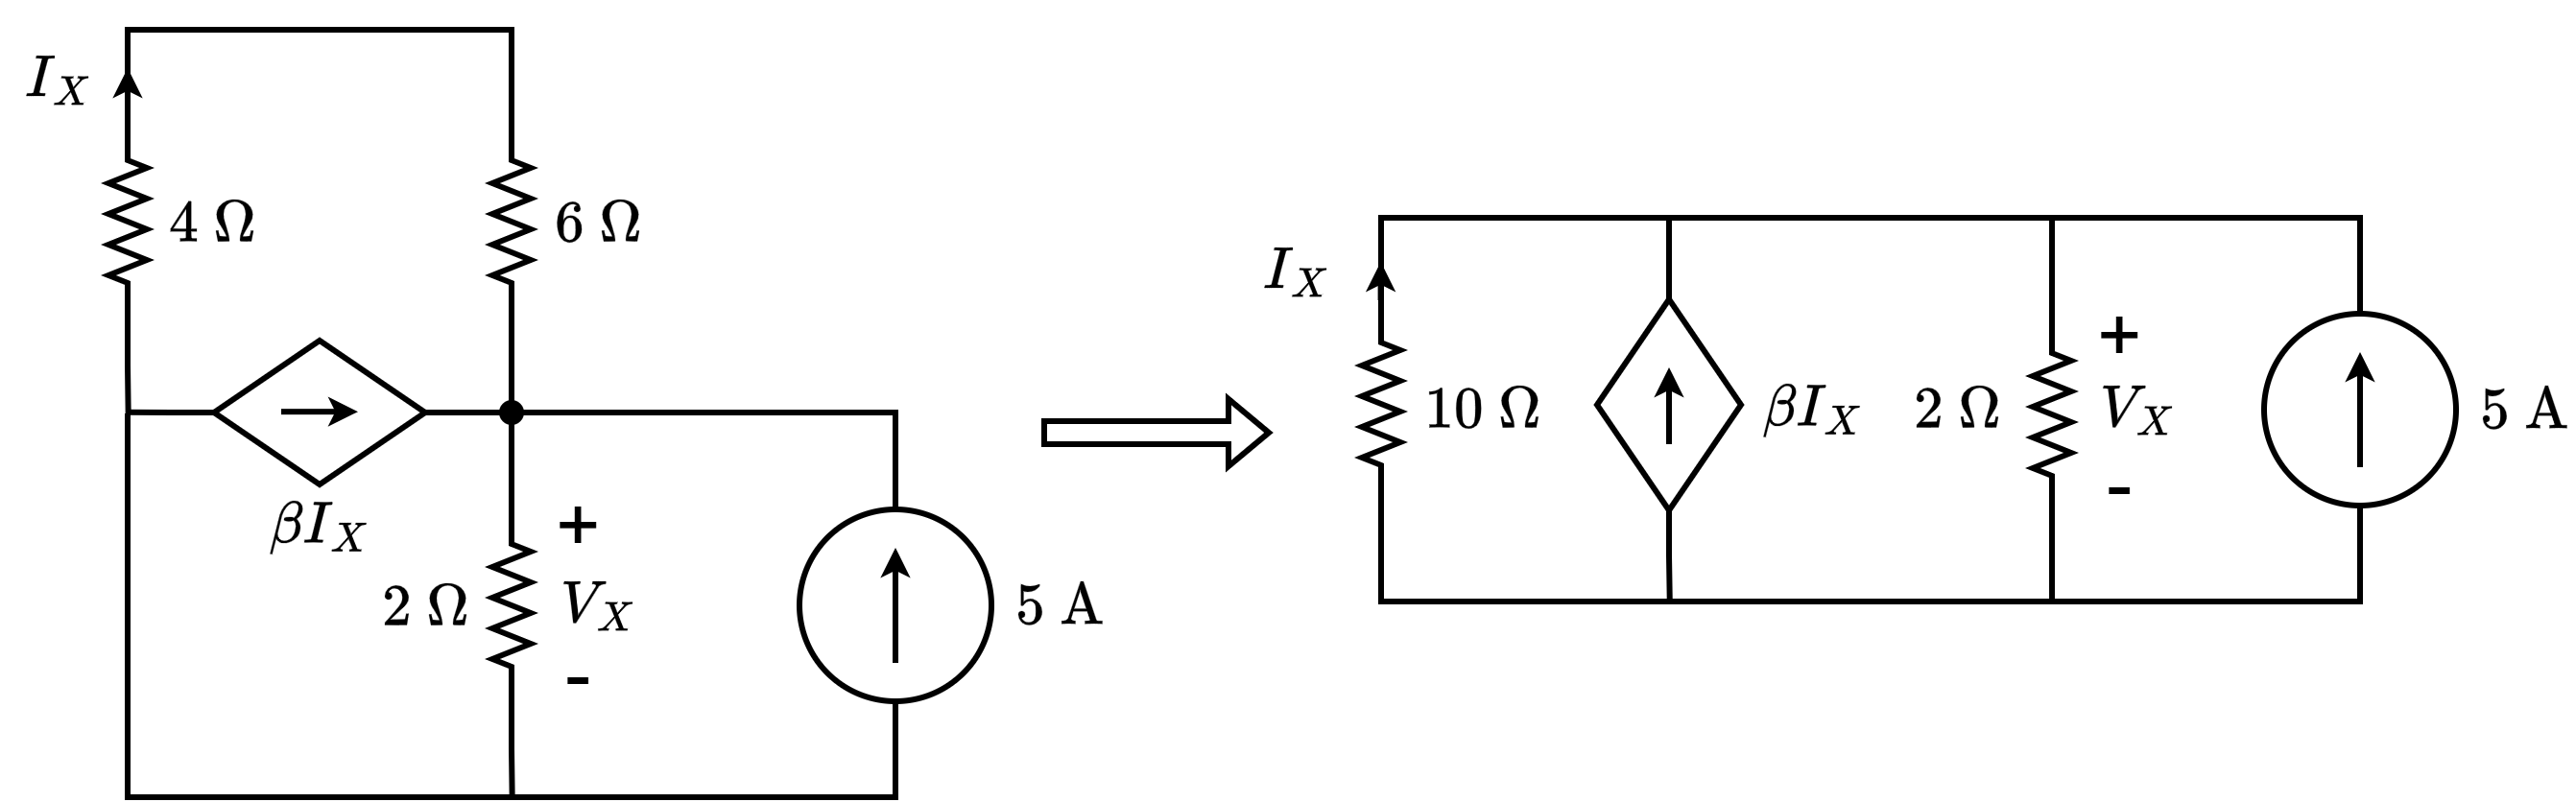
\includegraphics[width=0.9\textwidth]{super_5A.png}
\end{center}

Let's write our KCL at the top node. $I_X$ can be found with Ohm's law as $I_X = -V_X/10$. Substituting and crunching yields:
\begin{gather*}
0 = \frac{V_X}{2}  - I_X - \beta I_X -5 \\
5 = \frac{V_X}{2} - I_X(1+\beta) \\
5 = \frac{V_X}{2} + V_X\frac{1+\beta}{10} \\
V_X = \frac{5}{\frac{1}{2}+\frac{1+\beta}{10}} = \frac{50}{6+\beta}
\end{gather*}
Let's call this $V_{X\text{,5A}}(\beta)$ and save it for later.
\bigskip

\textbf{8 V source only:} open the 5 A source and short the 10 V source. Combine the resistors as before and the circuit can be rewritten as follows:
\begin{center}
    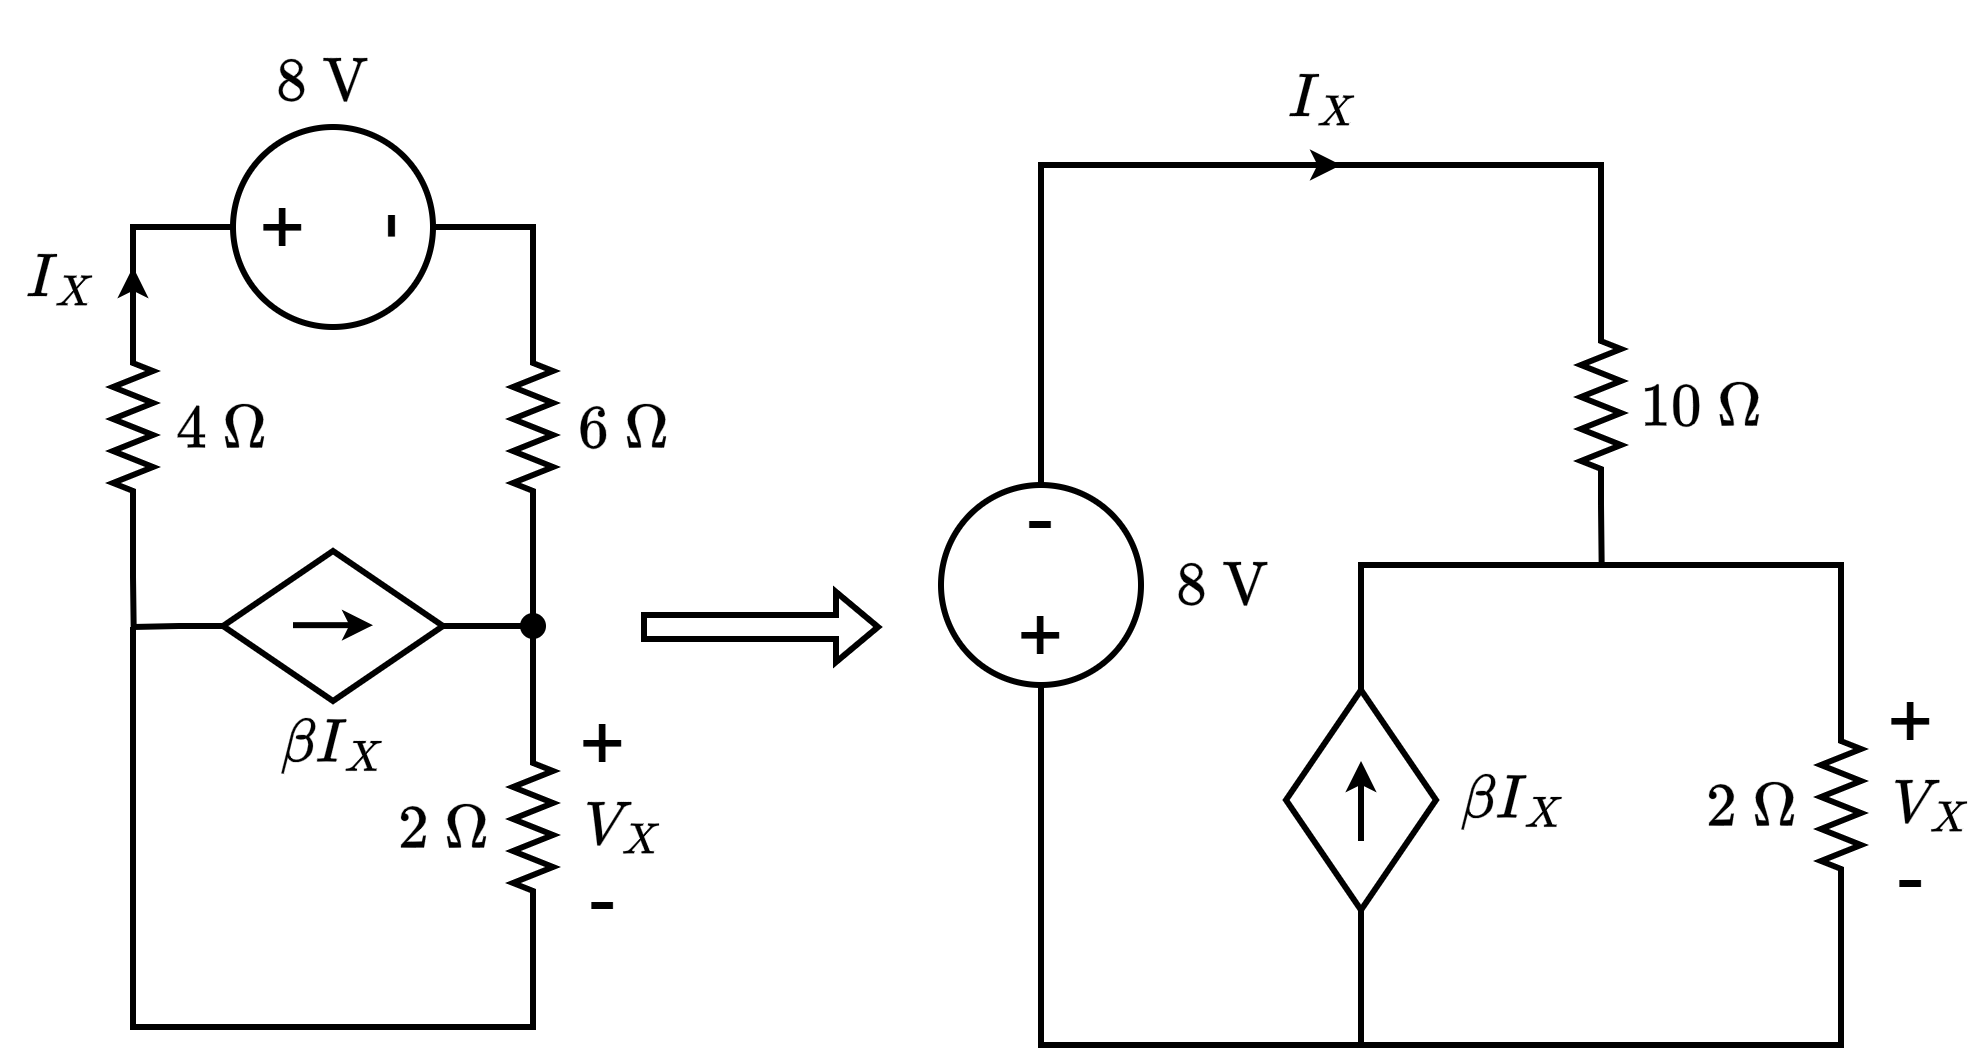
\includegraphics[width=0.9\textwidth]{super_8V.png}
\end{center}

 This can be solved as before using a KCL equation at the top of the \qty{2}{\ohm} resistor: \[\frac{V_X}{2} - I_X - \beta I_X = 0 \hspace{1cm} I_X = \frac{-8 - V_X}{10}\]
 Solving...
\begin{gather*}
\frac{V_X}{2} - I_X(1+\beta)= 0 \\
\frac{V_X}{2} +\frac{8 + V_X}{10}(1+\beta)= 0 \\
V_X\left(\frac{1}{2} + \frac{(1+\beta)}{10}\right) = -\frac{8(1+\beta)}{10} \\
V_X = \frac{-\frac{8(1+\beta)}{10}}{\frac{1}{2} + \frac{(1+\beta)}{10}} = \frac{-8(1+\beta)}{6+\beta}
\end{gather*}
Let's call this $V_{X\text{,8V}}(\beta)$ and save it for later.
\bigskip

\textbf{10 V source only:} open the 5 A source and short the 8 V source. Combine the resistors as before and the circuit can be rewritten as follows:
\begin{center}
    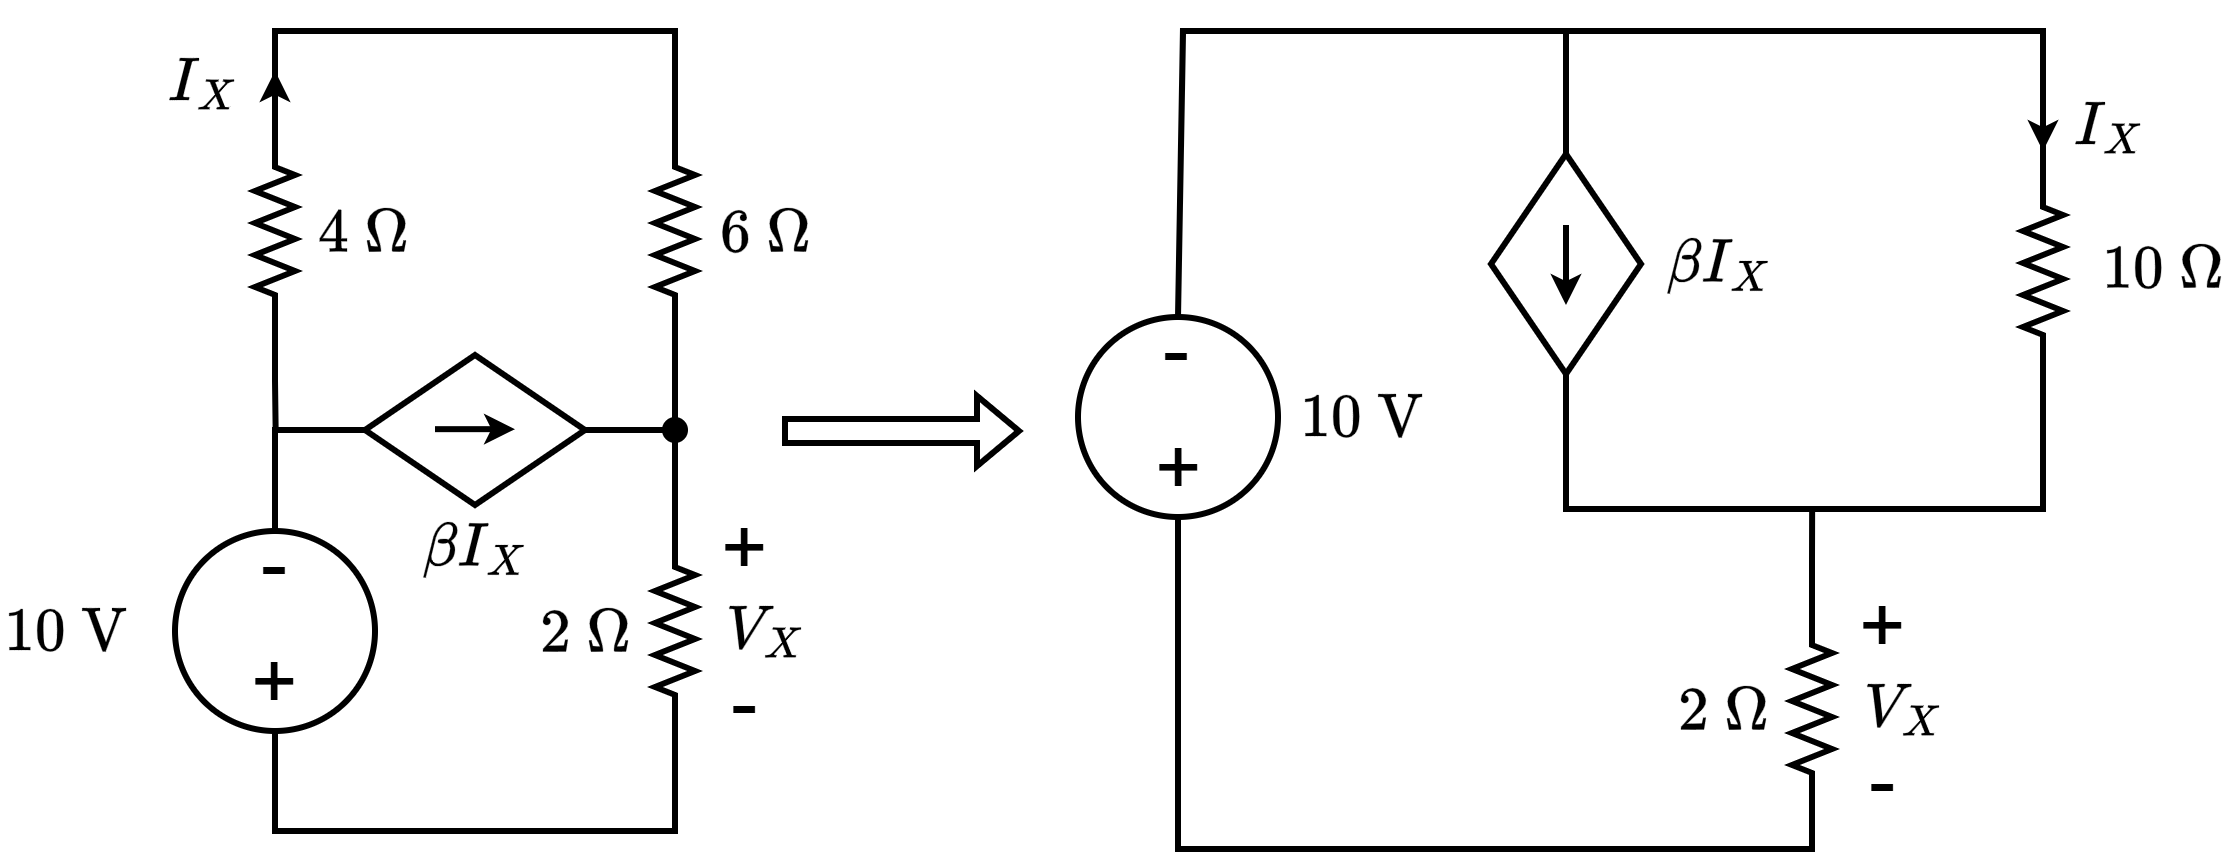
\includegraphics[width=0.9\textwidth]{super_10V.png}
\end{center}

This can be solved as before using a KCL equation at the top of the \qty{2}{\ohm} resistor: \[\frac{V_X}{2} - I_X - \beta I_X = 0 \hspace{1cm} I_X = \frac{-10 - V_X}{10}\]
Note that this is the same as the \qty{8}{\volt} equation except we are using \qty{-10}{\volt} instead. Replacing the voltage leads to...
\begin{gather*}
V_X\left(\frac{1}{2} + \frac{(1+\beta)}{10}\right) = -\frac{10(1+\beta)}{10} \\
V_X = \frac{-(1+\beta)}{\frac{1}{2} + \frac{(1+\beta)}{10}} = \frac{-10(1+\beta)}{6+\beta}
\end{gather*}
Let's call this $V_{X\text{,10V}}(\beta)$ and save it for later.
\bigskip
 
\textbf{Summation:}

Superposition tells us the final solutions is the addition of all three functions we derived:
\begin{align*}
V_X(\beta) &= V_{X\text{,5A}}(\beta) + V_{X\text{,8V}}(\beta) + V_{X\text{,10V}}(\beta) \\
V_X(\beta)&= \frac{50}{6+\beta} + \frac{-8(1+\beta)}{6+\beta} + \frac{-10(1+\beta)}{6+\beta} \\
V_X(\beta)&= \frac{50 - 18(1+\beta)}{6+\beta} = \frac{32 - 18\beta}{6+\beta}
\end{align*}
\end{answer}
\end{partquestion}

\begin{partquestion}{calculatevx}{Solve for $V_X$ given that $\beta = 0.25$}
\begin{answer}
Finding this is as simple as plugging in the given value of $\beta$.
\begin{align*}
    V_X(0.25)&= \frac{32 - 18\cdot0.25}{6+0.25} = \qty{4.4}{\volt}
\end{align*}
\end{answer}
\end{partquestion}

\begin{partquestion}{calculatek}{Find $\beta$ such that $V_X = \qty{17}{\volt}$}
\begin{answer}
This will require flipping the equation around to solve for $\beta$.
\begin{align*}
    V_X &= \frac{32 - 18\beta}{6+\beta} \\
    V_X(6+\beta) &= 32 - 18\beta \\
    \beta(18 + V_X) &= 32 - 6V_X \\
    \beta &= \frac{32 - 6V_X}{18 + V_X} \\
    \beta &= \frac{32 - 6\cdot17}{18 + 17} = -2 \\
\end{align*}
\end{answer}
\end{partquestion}

\begin{partquestion}{thev}{Find the equivalent resistance seen across $V_X$ in terms of $\beta$. What happens when $\beta = -6$? Use this to explain the result of $V_X(-6)$ from part (\cref{prob:controlledsourcegain:formulavx}).}

\begin{answer}
    We can find $R_{th}$ by disabling all independent sources and applying a test voltage and measuring the current that flows out of it. The ratio between these is the equivalent resistance! Since we are asked to find the equivalent resistance across $V_X$, we will attach our test source in parallel.
\begin{center}
    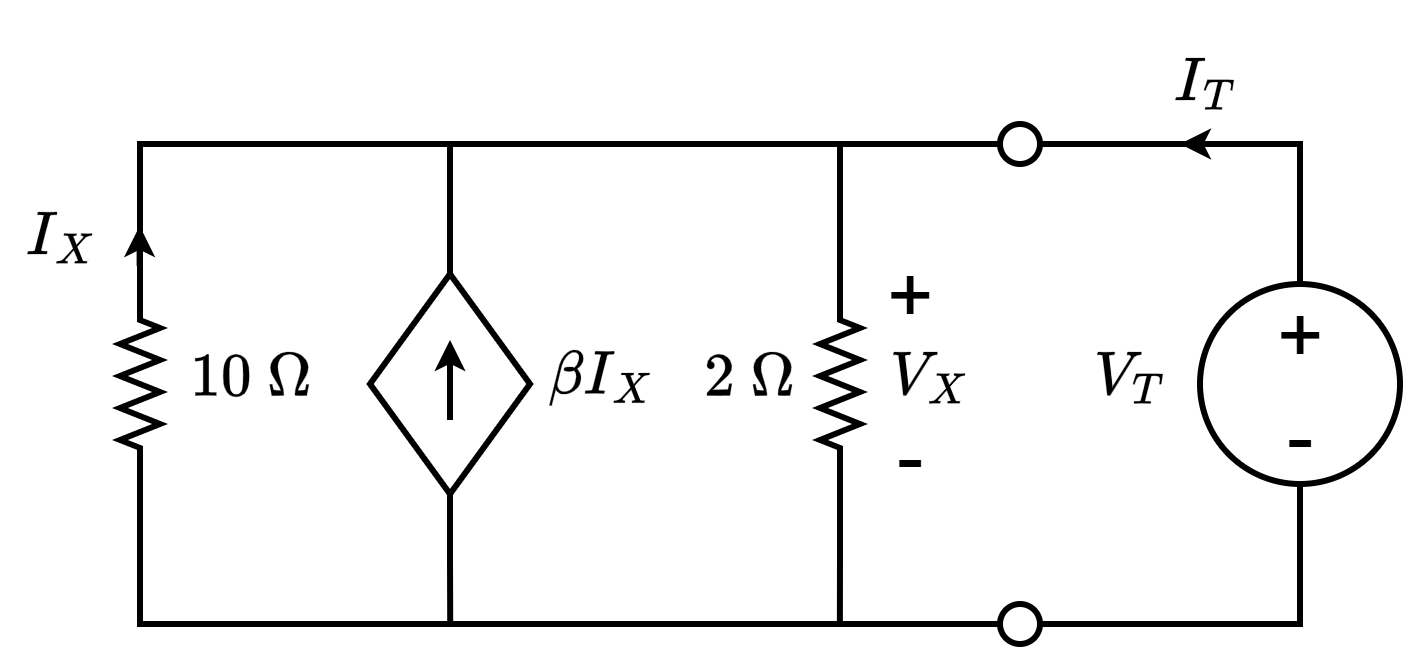
\includegraphics[width=0.9\textwidth]{rth.png}
\end{center}

Let's solve for $I_T$ using a KCL equation. Recall $V_X = V_T$.
\begin{align*}
    \frac{V_X}{2} - I_X - \beta I_X &= I_T \\
    \frac{V_T}{2} - I_X(1+\beta) &= I_T \\
    \frac{V_T}{2} - \left(-\frac{V_T}{10}\right)(1+\beta) &= I_T \\
    V_T\left(\frac{1}{2} + \frac{1+\beta}{10}\right) &= I_T \\
\end{align*}
We can then find $R_{th} = V_T/I_T$:
\begin{align*}
    R_{th} = \frac{V_T}{I_T} &= \frac{1}{\frac{1}{2} + \frac{1+\beta}{10}} \\
    R_{th} &= \frac{10}{5 + (1+\beta)} \\
    R_{th} &= \frac{10}{6+\beta} \\
\end{align*}
We have now found the equivalent resistance in terms of the current gain $\beta$. When the current gain $\beta = -6$, the formula predicts $R_{th} = \infty$, an open circuit. The dependent current source provides just enough current to satisfy the \qty{10}{\ohm} and \qty{2}{\ohm} resistor at any voltage, so there isn't any room for an ideal source to supply or draw any additional current $I_T$. The formula from part (\cref{prob:controlledsourcegain:formulavx}):
\[
V_X = \frac{32 - 18\beta}{6+\beta}
\]
shows that $V_X$ also blows up to infinity when $\beta = -6$. This makes senses because we have a \qty{5}{\ampere} source trying to drive current into our open load. Ohm's law suggests $V = I\cdot R$, so $V_X = 5 \cdot \infty = \infty$.
    
\end{answer}
\end{partquestion}

\end{mainquestion}
